\section{ОБЗОР ПРЕДМЕТНОЙ ОБЛАСТИ}

%Обзор состояния рассматриваемого в ВКР вопроса на основании изучения литературных источников.

Наиболее универсальным прибором для измерений параметров волоконно-оптических линий связи (\acrshort{волс}) является оптический рефлектометр во временной области (\acrshort{ор}), работа которого основана на методе обратного рассеяния (\acrshort{мор}).

Рассеяние света происходит на флуктуациях показателя преломления кварцевого стекла, застывших при вытяжке волокна. Размер этих неоднородностей (релеевских центров) мал по сравнению с длиной волны и свет на них рассеивается во все стороны, в том числе и назад в моду волокна (рис. \ref{ris:obr_rass}).

\begin{figure}[h]
  \center{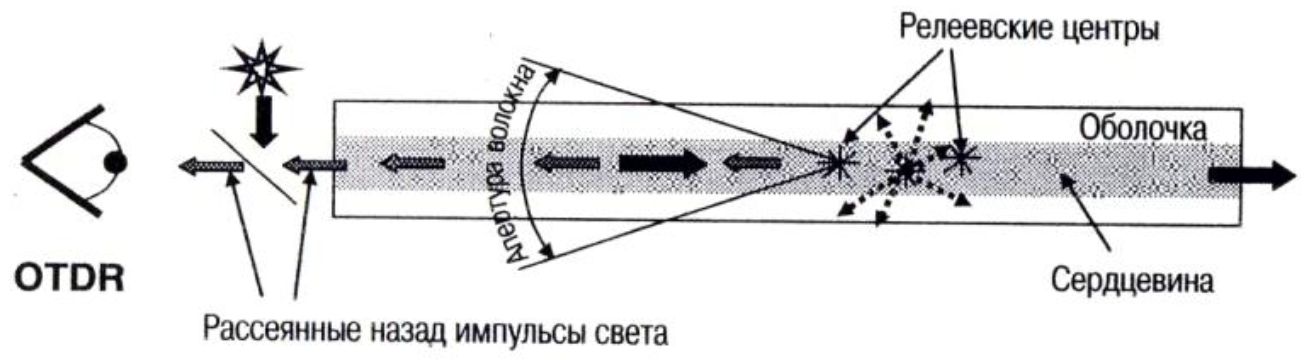
\includegraphics[width=\linewidth]{obr_rass}}
  \caption{В \acrshort{ор} приходят импульсы света рассеянные назад в моду волокна}
  \label{ris:obr_rass}
\end{figure}

Релеевские центры распределены однородно вдоль волокна, и в рассеянной на них волне содержится информация обо всех параметрах линии, влияющих на поглощение света. Именно за счет детектирования рассеянного излучения удается обнаруживать неотражающие (поглощающие) неоднородности в волокне. Например, по сигналу обратного релеевского рассеяния света можно измерить распределение потерь в строительных длинах оптических кабелей и потери в сростках волокон.

\acrshort{мор} основан на введении в \acrshort{ов} импульсного оптического излучения и последующем анализе сигнала обратного рассеяния (\acrshort{сор}), который возвращается на фотоприемное устройство (\acrshort{фпу}). В результате математической обработки \acrshort{сор} на экране \acrshort{ор} формируется изображение, называемое рефлектограммой и представляющее собой зависимость уровня \acrshort{сор} от расстояния вдоль линейного волоконного тракта~\cite{bogdanova:reflectometria}.

Угол наклона участков рефлектограммы между пиками характеризует погонное затухание по длине кабеля. Если в сегменте везде используется волокно одного и того же типа и качества, все участки рефлектограммы, снятой на одной длине волны, должны иметь одинаковый наклон.

\subsection{Устройство рефлектометра}

В большинстве моделей \acrshort{ор} используется модульная конструкция (рис.~\ref{ris:otdr_schematic}). Она содержит базовый модуль и несколько сменных оптических модулей. Базовый модуль представляет собой персональный компьютер, приспособленный для обработки сигнала и вывода его на дисплей. Оптический модуль включает в себя лазерный диод, фотоприемник, оптический ответвитель и оптический разъем. Стоимость оптического модуля зависит от величины его динамического диапазона и может в несколько раз превышать стоимость базового модуля. Модульная конструкция \acrshort{ор} позволяет потребителю не только выбрать необходимую ему на данный момент конфигурацию прибора, но и в дальнейшем модернизировать прибор, например, установив, многомодовый модуль или одномодовый модуль с большим динамическим диапазоном.

\begin{figure}[h]
  \center{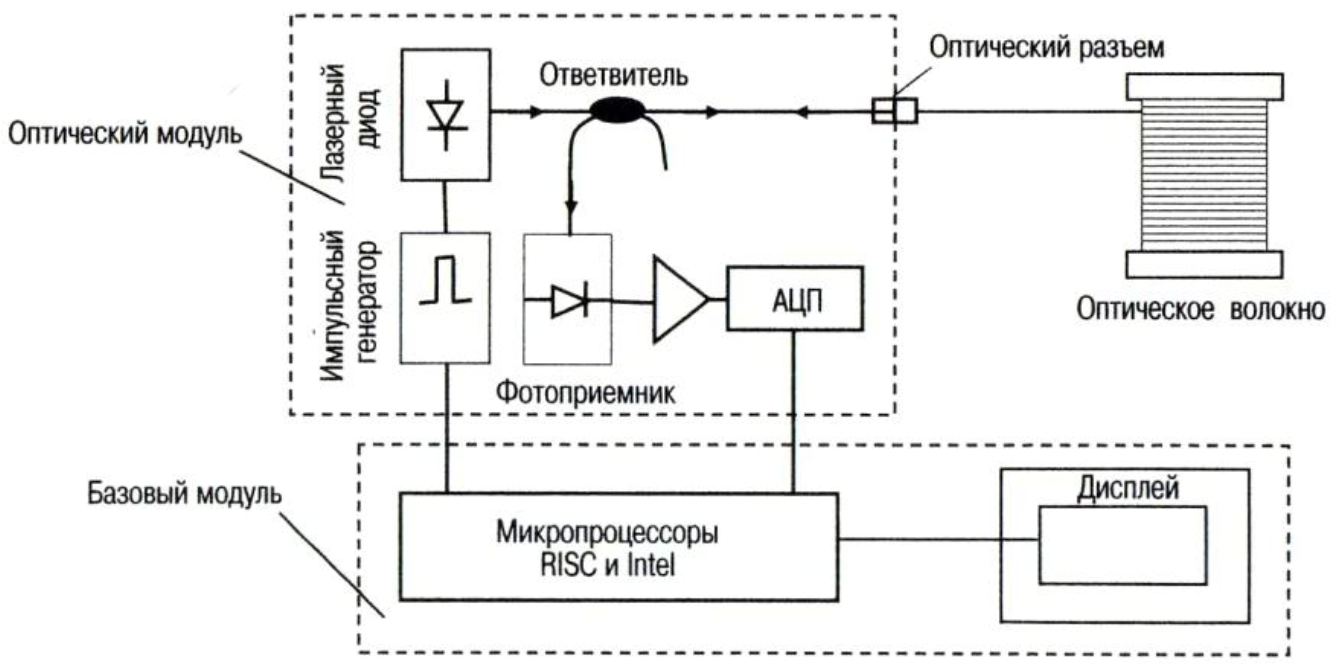
\includegraphics[width=\linewidth]{otdr_schematic}}
  \caption{Блок схема \acrshort{ор}}
  \label{ris:otdr_schematic}
\end{figure}

В качестве источника излучения в оптическом модуле обычно используется лазерные диоды типа Фабри-Перо, наибольшая же мощность излучения (и, соответственно, динамический диапазон рефлектометра) достигается с помощью лазерных диодов с квантовыми ямами. С их помощью генерируются импульсы мощностью 10\dots1000 мВт, длительностью от 2 нс\dots20 мкc и частотой повторения несколько килогерц. Эти импульсы поступают через ответвитель на оптический разъем, к которому подключается исследуемое волокно. Рассеянные в волокне импульсы света возвращаются в оптический модуль и передаются с помощью ответвителя на фотоприемник (лавинный фотодиод), где они преобразуются в электрический сигнал. Этот сигнал усиливается, накапливается, обрабатывается в базовом модуле и отображается на дисплее в графической форме в виде рефлектограммы. Такое представление информации позволяет анализировать её как визуально, так и автоматически с помощью встроенных программных алгоритмов~\cite{listvin:reflectometria}.

\subsection{События на линии}

\acrshort{ор} позволяет находить и отображать на рефлектограмме сварные и механические соединения, коннекторные соединения, изгибы и другие неоднородности волокна. Такие неоднородности называют событиями. 
События могут быть \textbf{отражающими} и \textbf{неотражающими}. 

Потери в разъемных соединениях являются следствием несовершенства как самой конструкции соединителя, так и процесса оконцовывания \acrshort{ов}. Потери в разъемных соединениях зависят от неточности юстировки волокон при их заделке в наконечник соединителя (радиальное, угловое и осевое смещение) и некачественной обработки (полировки) торцов соединяемых \acrshort{ов}. В разъемных соединениях эти потери обычно являются основными.

Потери в неразъемных соединениях определяются неточностью
юстировки \acrshort{ов} в сварочном аппарате перед сваркой. Однако современные сварочные аппараты имеют автоматическую юстировку и автоматическое управление процессом сварки \acrshort{ов}, обеспечивающее минимальные потери. Вследствие этого потери в сварке в основном определяются различием параметров свариваемых \acrshort{ов}~\cite{bilina:izmerenie_parametrov}.

Коннекторные соединения, трещина в волокне или обрыв, образующие поверхность разлома под углом порядка 90º к оси волокна --- примеры отражающих неоднородностей. В этих случаях происходит отражение части исходного излучения в направлении \acrshort{фпу}. На рефлектограмме такие события отображаются в виде пиков. 
Отражающие неоднородности сопровождаются возвратными потерями, которые могут быть рассчитаны по выражению (\ref{eqn:refl_loss}).

\begin{equation}
  \label{eqn:refl_loss}
  \alpha=-10\cdot \lg R
\end{equation}

\noindent где \\
$R$~--- коэффициент отражения.

В отличие от отражающих неоднородностей, в неразъемных соединениях (сварные, клеевые и механические сростки волокон), как правило нет воздушного зазора и отсутствуют отражения. Они отображаются на рефлектограмме ступенькой.

\subsection{Обзор формата SOR (Telecordia SR-4731)}

Наиболее распространенным форматом для хранения результатов измерения оптических рефлектометров является формат SOR (Standard OTDR Record) Telecordia SR-4731.
Он читается всеми приложениями для обработки рефлектограмм. Альтернативным форматом является TRC, с ним в частности работают приборы компании EXFO~\cite{web:volsexpert_reflectometria}.

Данный стандарт предусматривает следующие блоки~\cite{web:otdr_format}:

\subsubsection{Блок общих параметров}

Блок состоит из следующих полей:
\begin{itemize}
  \item id кабеля;
  \item id \acrshort{ов};
  \item тип \acrshort{ов};
  \item длина волны;
  \item точка А;
  \item точка Б;
  \item код кабеля;
  \item состояние кабеля, одно из значений:
  \begin{itemize}
    \item \textbf{BC}: как проложен;
    \item \textbf{CC}: текущее;
    \item \textbf{RC}: после ремонта;
    \item \textbf{OT}: иное.
  \end{itemize}
  \item пользовательский отступ;
  \item расстояние до пользовательского отступа;
  \item оператор;
  \item комментарии.
\end{itemize}

\subsubsection{Блок поставщика оптического рефлектометра}

Блок состоит из следующих полей:
\begin{itemize}
  \item наименование поставщика;
  \item наименование \acrshort{ор};
  \item серийный номер \acrshort{ор};
  \item название модуля;
  \item серийный номер модуля;
  \item версия \acrshort{по};
  \item прочее.
\end{itemize}

\subsubsection{Блок фиксированных параметров}
\label{fixed_params_block}

Блок состоит из следующих полей:
\begin{itemize}
  \item дата и время создания рефлектограммы (количество секунд прошедших с 1 января 1970 г.);
  \item единицы измерения, одно из значений:
  \begin{itemize}
    \item \textbf{km}: километры;
    \item \textbf{mt}: метры;
    \item \textbf{ft}: футы;
    \item \textbf{kf}: килофуты;
    \item \textbf{mi}: мили.
  \end{itemize}
  \item количество длин пульсов (на случай, если в файле несколько рефлектограмм);
  \item длина пульса (повторяется столько раз, сколько указано в пункте выше) (нс);
  \item разброс между измерений (делить на $10$, чтобы получить фс);
  \item количество измерений;
  \item показатель преломления;
  \item коэффициент обратного рассеяния (умножить на $-0,1$, чтобы получить дБ);
  \item время усреднения (с);
  \item дальность (умножить на $2\cdot 10^{-5}$, чтобы получить км);
  \item уровень шума;
  \item порог потерь (умножить на $0,001$, чтобы получить дБ);
  \item порог отражения (умножить на $-0,001$, чтобы получить дБ);
  \item порог конца передачи (умножить на $0,001$, чтобы получить дБ);
  \item тип рефлектограммы, одно из значений:
  \begin{itemize}
    \item \textbf{ST}: стандартная рефлектограмма;
    \item \textbf{RT}: обратная рефлектограмма;
    \item \textbf{DT}: разница рефлектограмм;
    \item \textbf{RF}: образец.
  \end{itemize}
\end{itemize}

\subsubsection{Блок ключевых событий}

Cледующие поля повторяются для каждого события:
\begin{itemize}
  \item номер события;
  \item время до события (умножить на $0,1$, чтобы получить нс);
  \item затухание (умножить на $0,001$, чтобы получить дБ/км);
  \item потери сварки (умножить на $0,001$, чтобы получить дБ);
  \item потери отражения (умножить на $0,001$, чтобы получить дБ);
  \item тип события, одно из полей:
  \begin{itemize}
    \item \textbf{0}: ступенька вверх или вниз;
    \item \textbf{1}: отражение;
    \item \textbf{2}: множественное событие.
  \end{itemize}
  \item конец предыдущего события (0, если первое событие);
  \item начало события;
  \item конец события;
  \item начало следующего события (равно дальности, если последнее событие);
  \item пик текущего события;
  \item комментарий.
\end{itemize}

После ключевых событий следующий блок значений:
\begin{itemize}
  \item суммарное затухание (умножить на $0,001$, чтобы получить дБ);
  \item начало \acrshort{ов};
  \item протяженность \acrshort{ов};
  \item потери отражения (умножить на $0,001$, чтобы получить дБ).
\end{itemize}

Зная время до события можно рассчитать расстояние до него по формуле~(\ref{eqn:event_distance})

\begin{equation}
  \label{eqn:event_distance}
  d = t \cdot \frac{c}{n}
\end{equation}

\noindent где \\
$t$~--- время до события \\
$c$~--- скорость света \\
$n$~--- показатель преломления

\subsubsection{Блок точек}

В начале блока идет количество точек (совпадает с количеством измерений указанным в пункте \ref{fixed_params_block}), после этого идет количество рефлектограмм (совпадает с количеством длин пульсов указанным в пункте \ref{fixed_params_block}). Далее идут измерения~--- дБ и соответственные расстояния.

\subsubsection{Блок контрольной суммы}

Контрольная сумма вычисленная по алгоритму CRC-16.

\subsection{Анализ существующих решений}

Распространенные в данный момент аналоги не является кросс платформенными, что значит они не имееют возможность выполняться во всех популярных операционных системах (Window, OSX, Linux) и на всех поддерживаемых этими платформами архитектурах.

\subsubsection{EXFO FastReporter и EXFO LiteReporter}

\textbf{Ключевой функционал:} \cite{web:fastreporter_specs}
\begin{itemize}
  \item автопоиск событий;
  \item создание эталонных рефлектограмм;
  \item обработка наборов рефлектограмм;
  \item двунапраленный анализ;
  \item интеграция с облачными сервисами.
\end{itemize}

Поддерживаемые операционные системы: \textbf{Windows}.

\begin{figure}[H]
  \center{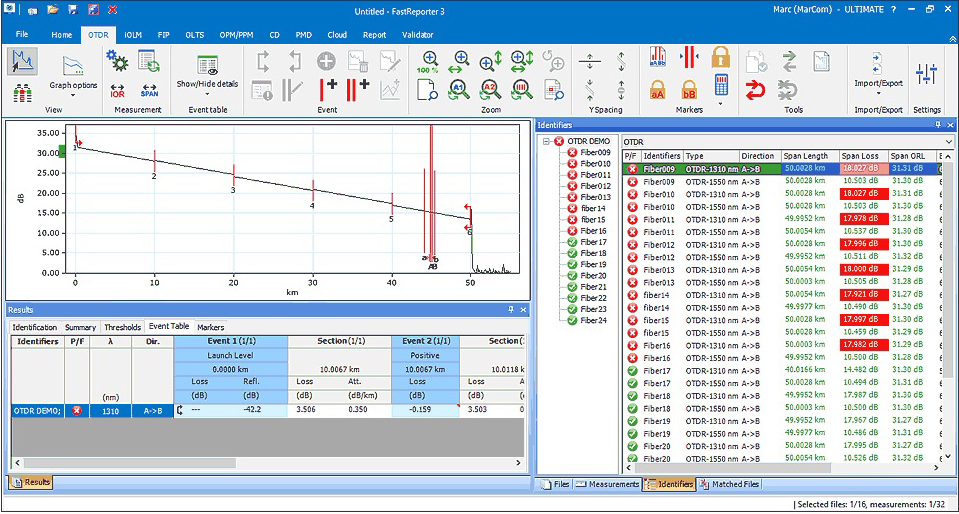
\includegraphics[width=\linewidth]{fastreporter}}
  \caption{Интерфейс программы FastReporter}
  \label{ris:fastreporter}
\end{figure}

\subsubsection{VIAVI Solutions Fiber Trace Viewer}

\textbf{Ключевой функционал:} \cite{web:viavi}
\begin{itemize}
  \item автопоиск событий;
  \item обработка наборов рефлектограмм;
  \item двунапраленный анализ.
\end{itemize}

Поддерживаемые операционные системы: \textbf{Windows}.

\subsubsection{Yokogawa Electric Corporation AQ 7933}

\textbf{Ключевой функционал:} \cite{web:yokogawa}
\begin{itemize}
  \item автопоиск событий;
  \item обработка наборов рефлектограмм;
  \item двунапраленный анализ;
  \item создание событий.
\end{itemize}

Поддерживаемые операционные системы: \textbf{Windows}.

\begin{figure}[H]
  \center{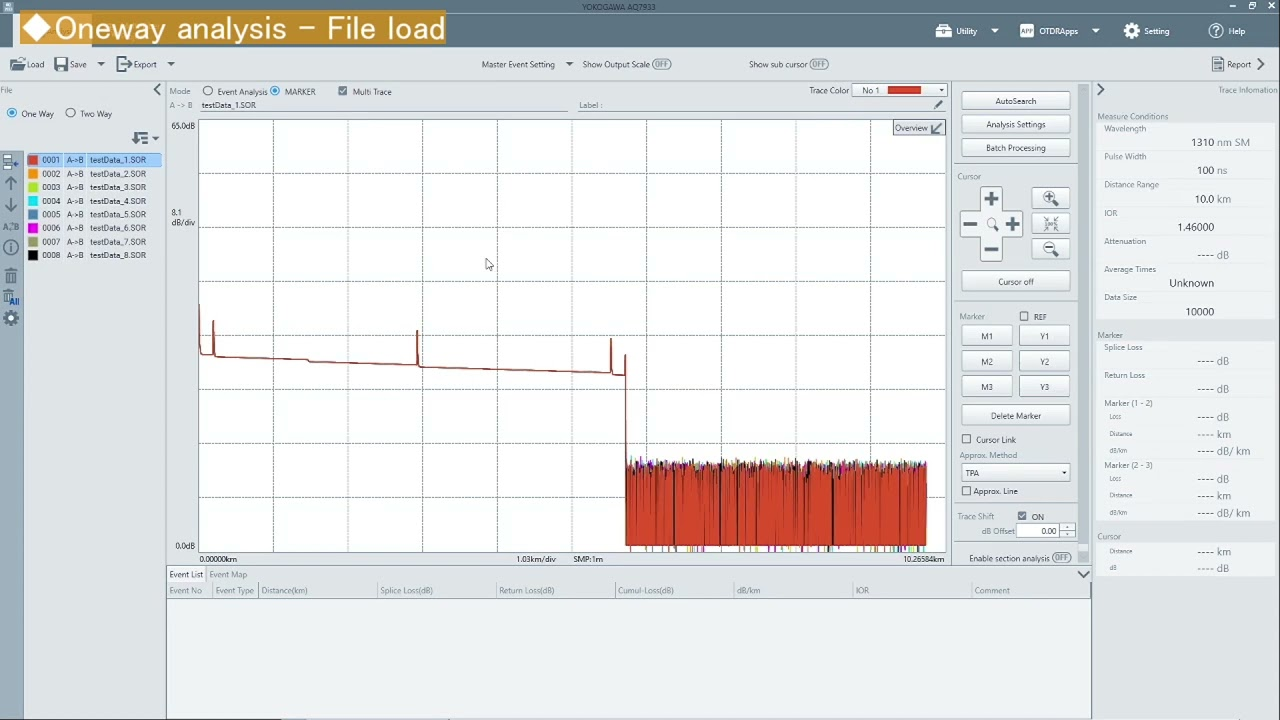
\includegraphics[width=\linewidth]{Yokogawa_Electric_Corporation_AQ_7933}}
  \caption{Интерфейс программы Yokogawa Electric Corporation AQ 7933}
  \label{ris:yokogawa}
\end{figure}

\subsubsection{СвязьСервис TopOTDRViewer}

\textbf{Ключевой функционал:} \cite{web:topotdrviewer}
\begin{itemize}
  \item автопоиск событий;
  \item обработка наборов рефлектограмм.
\end{itemize}

Поддерживаемые операционные системы: \textbf{Windows}.

\begin{figure}[H]
  \center{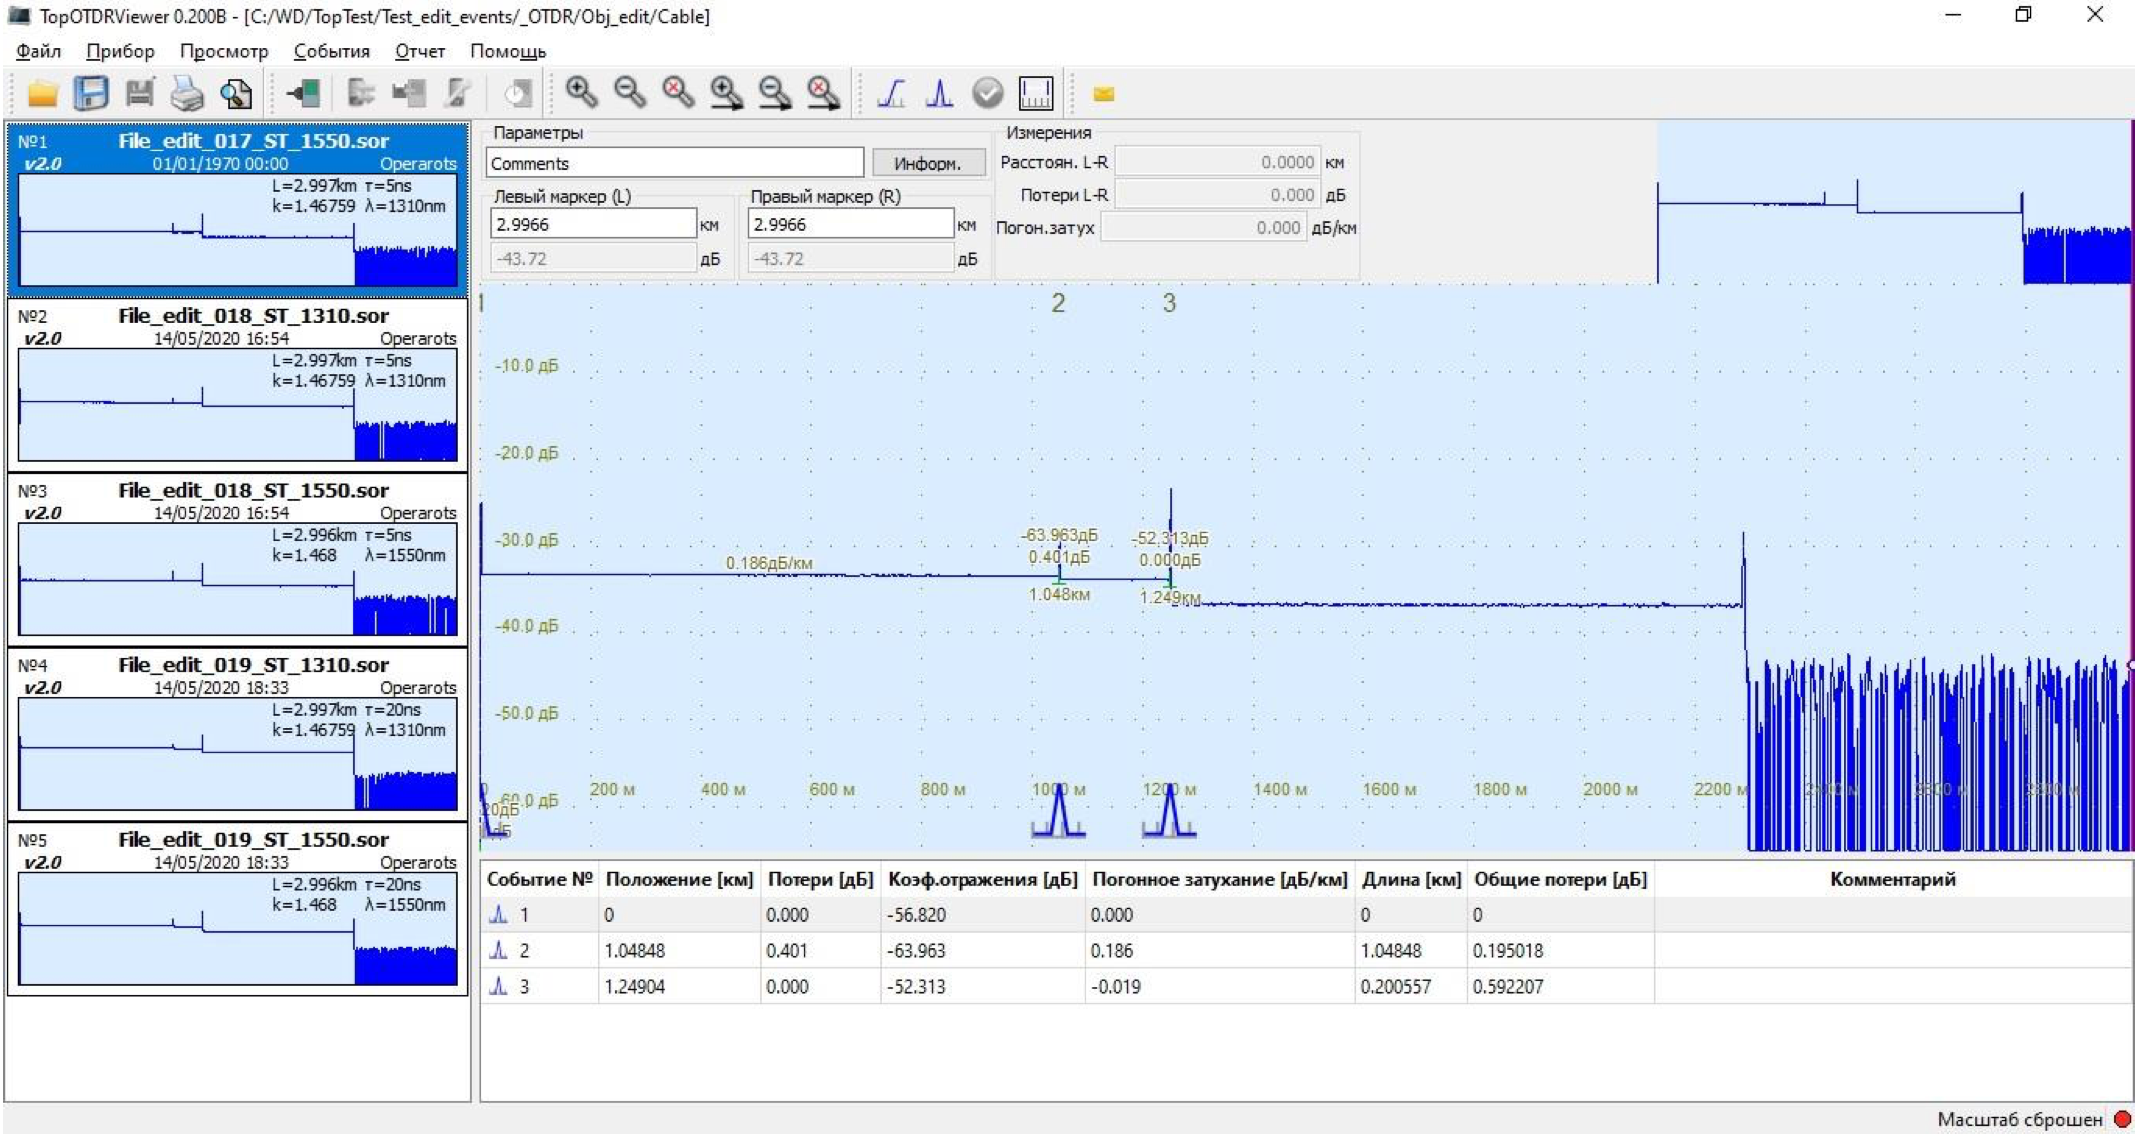
\includegraphics[width=\linewidth]{topotdrviewer}}
  \caption{Интерфейс программы TopOTDRViewer}
  \label{ris:topotdrviewer}
\end{figure}

\subsubsection{SORTraceViewer}

\textbf{Ключевой функционал:} \cite{web:sortraceviewer}
\begin{itemize}
  \item автопоиск событий;
  \item двунапраленный анализ;
  \item обработка наборов рефлектограмм;
  \item редактирование точек рефлектограммы.
\end{itemize}

Поддерживаемые операционные системы: \textbf{Windows}, \textbf{Linux}.

\begin{figure}[H]
  \center{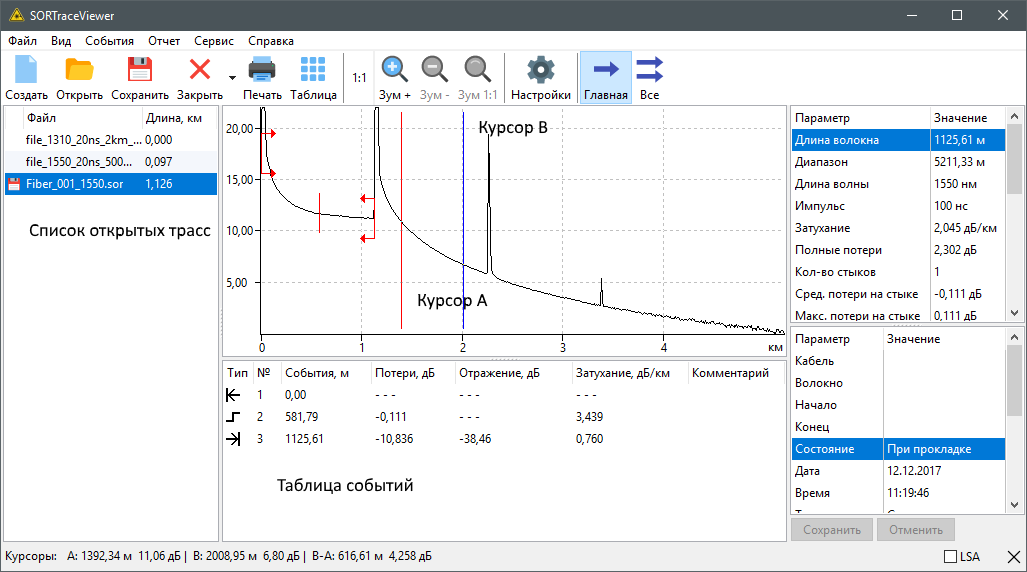
\includegraphics[width=\linewidth]{sortraceviewer}}
  \caption{Интерфейс программы SORTraceViewer}
  \label{ris:sortraceviewer}
\end{figure}

\subsection{Выводы по разделу}

В разделе описана предметная область, рассмотрено устройство рефлектометра, а также формат данных в которых сохраняются результаты измерения. Помимо этого рассмотрены существующие программы для обработки результатов измерений \acrshort{ор}.
